\begin{frame}{Variational Inference \citep{jordan:1998:variational}}

Variational inference is an {\color{blue} expansion-based methodology}

\begin{itemize}
\item \emph{Example}: algebraic vs.\ variational definition of the maximum eigenvalue
\[
A x = \lambda x
\ \ \ \ vs.\ \ \ \
\lambda = \max_x \left\{ \frac{x^T A x}{x^T x} \right\}
\]
\end{itemize}

In general, we define an object (e.g., an integral) via an {\color{blue} optimization problem}, using {\color{blue} test functions} to obtain necessary conditions for optimality

E.g., likelihood-based objects naturally lend themselves to optimization problems involving the KL divergence, with the test functions being exponential-family densities

Here we go further, using test functions to probe sensitivities in function spaces of interest

\end{frame}

\begin{frame}{Variational Stick-Breaking \citep{blei:2006:variationalbnp}}

Let $\zeta$ denote all model variable, including stick lengths 
$\nu = (\nu_1, \nu_2, ...)$.   
Let $\x$ denote the observed data.  The posterior $\p(\zeta | \x)$ is intractable.

We approximate $\p(\zeta \vert \z)$ using distributions $\q(\zeta \vert \eta)$,
parameterized by a finite-dimensional $\eta \in \etadom \subseteq
\mathbb{R}^{\etadim}$. 
We solve
\begin{align*}
\etaopt :={} \argmin_{\eta \in \etadom}  \KL{\eta}
\quad\textrm{where}\quad
\KL{\eta} :={} \KL{\q(\zeta \vert \eta) || \p(\zeta \vert \x)} 
\end{align*}
%\pause
\textbf{Note:}

\begin{itemize}
\item The optimal variational parameters $\etaopt$ depend on the prior through optimizing the KL objective.

\item The approximate posterior quantities are then functions of $\etaopt$, e.g.\
\end{itemize}

\begin{minipage}{0.4\textwidth}
\centering
$\etaopt \mapsto
\expect{\q(\zeta \vert \etaopt)}{\#\text{clusters}}
\quad$
\end{minipage}
\begin{minipage}{0.05\textwidth}
or
\end{minipage}
\begin{minipage}{0.12\textwidth}
\begin{flushright}
$\etaopt \mapsto$
\end{flushright}
\end{minipage}
\begin{minipage}{0.22\textwidth}
\begin{flushleft}
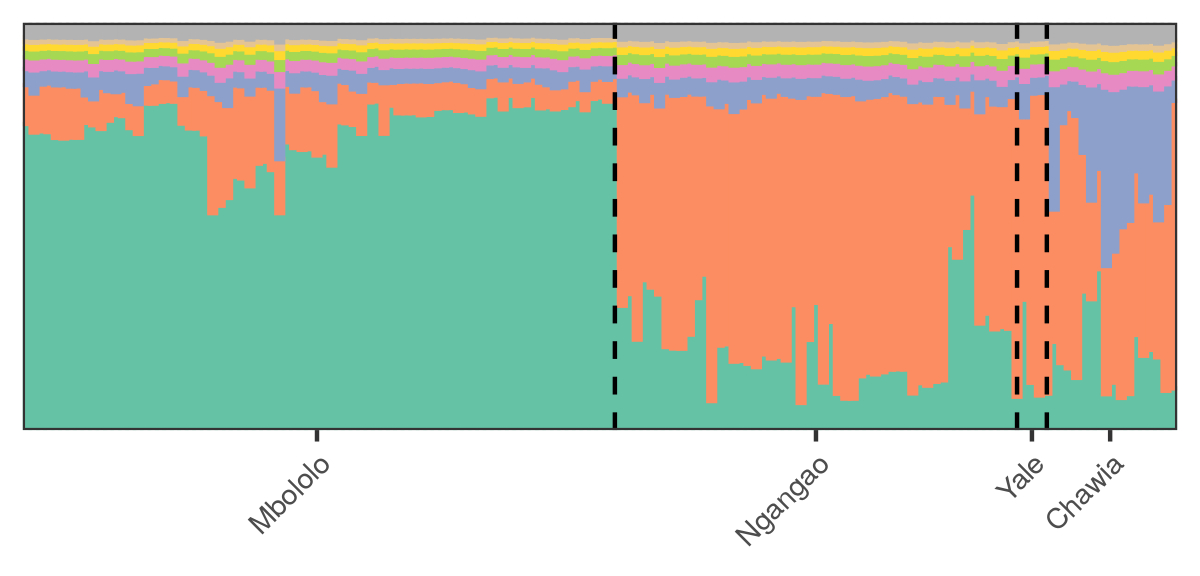
\includegraphics[width = 3cm]{./figure/structure_init-1.png}
\end{flushleft}
\end{minipage}

%\pause 
\begin{mdframed}[style=MyFrame]
\begin{center}
{\bf How do these approximate posterior quantities depend on the stick-breaking prior?}
\end{center}
\end{mdframed}

\end{frame}
